\documentclass{standalone}
\usepackage{tikz}
\usetikzlibrary{patterns, positioning}
\usepackage[sfdefault]{ClearSans} %% option 'sfdefault' activates Clear Sans as the default text font
\usepackage[T1]{fontenc}

\begin{document}
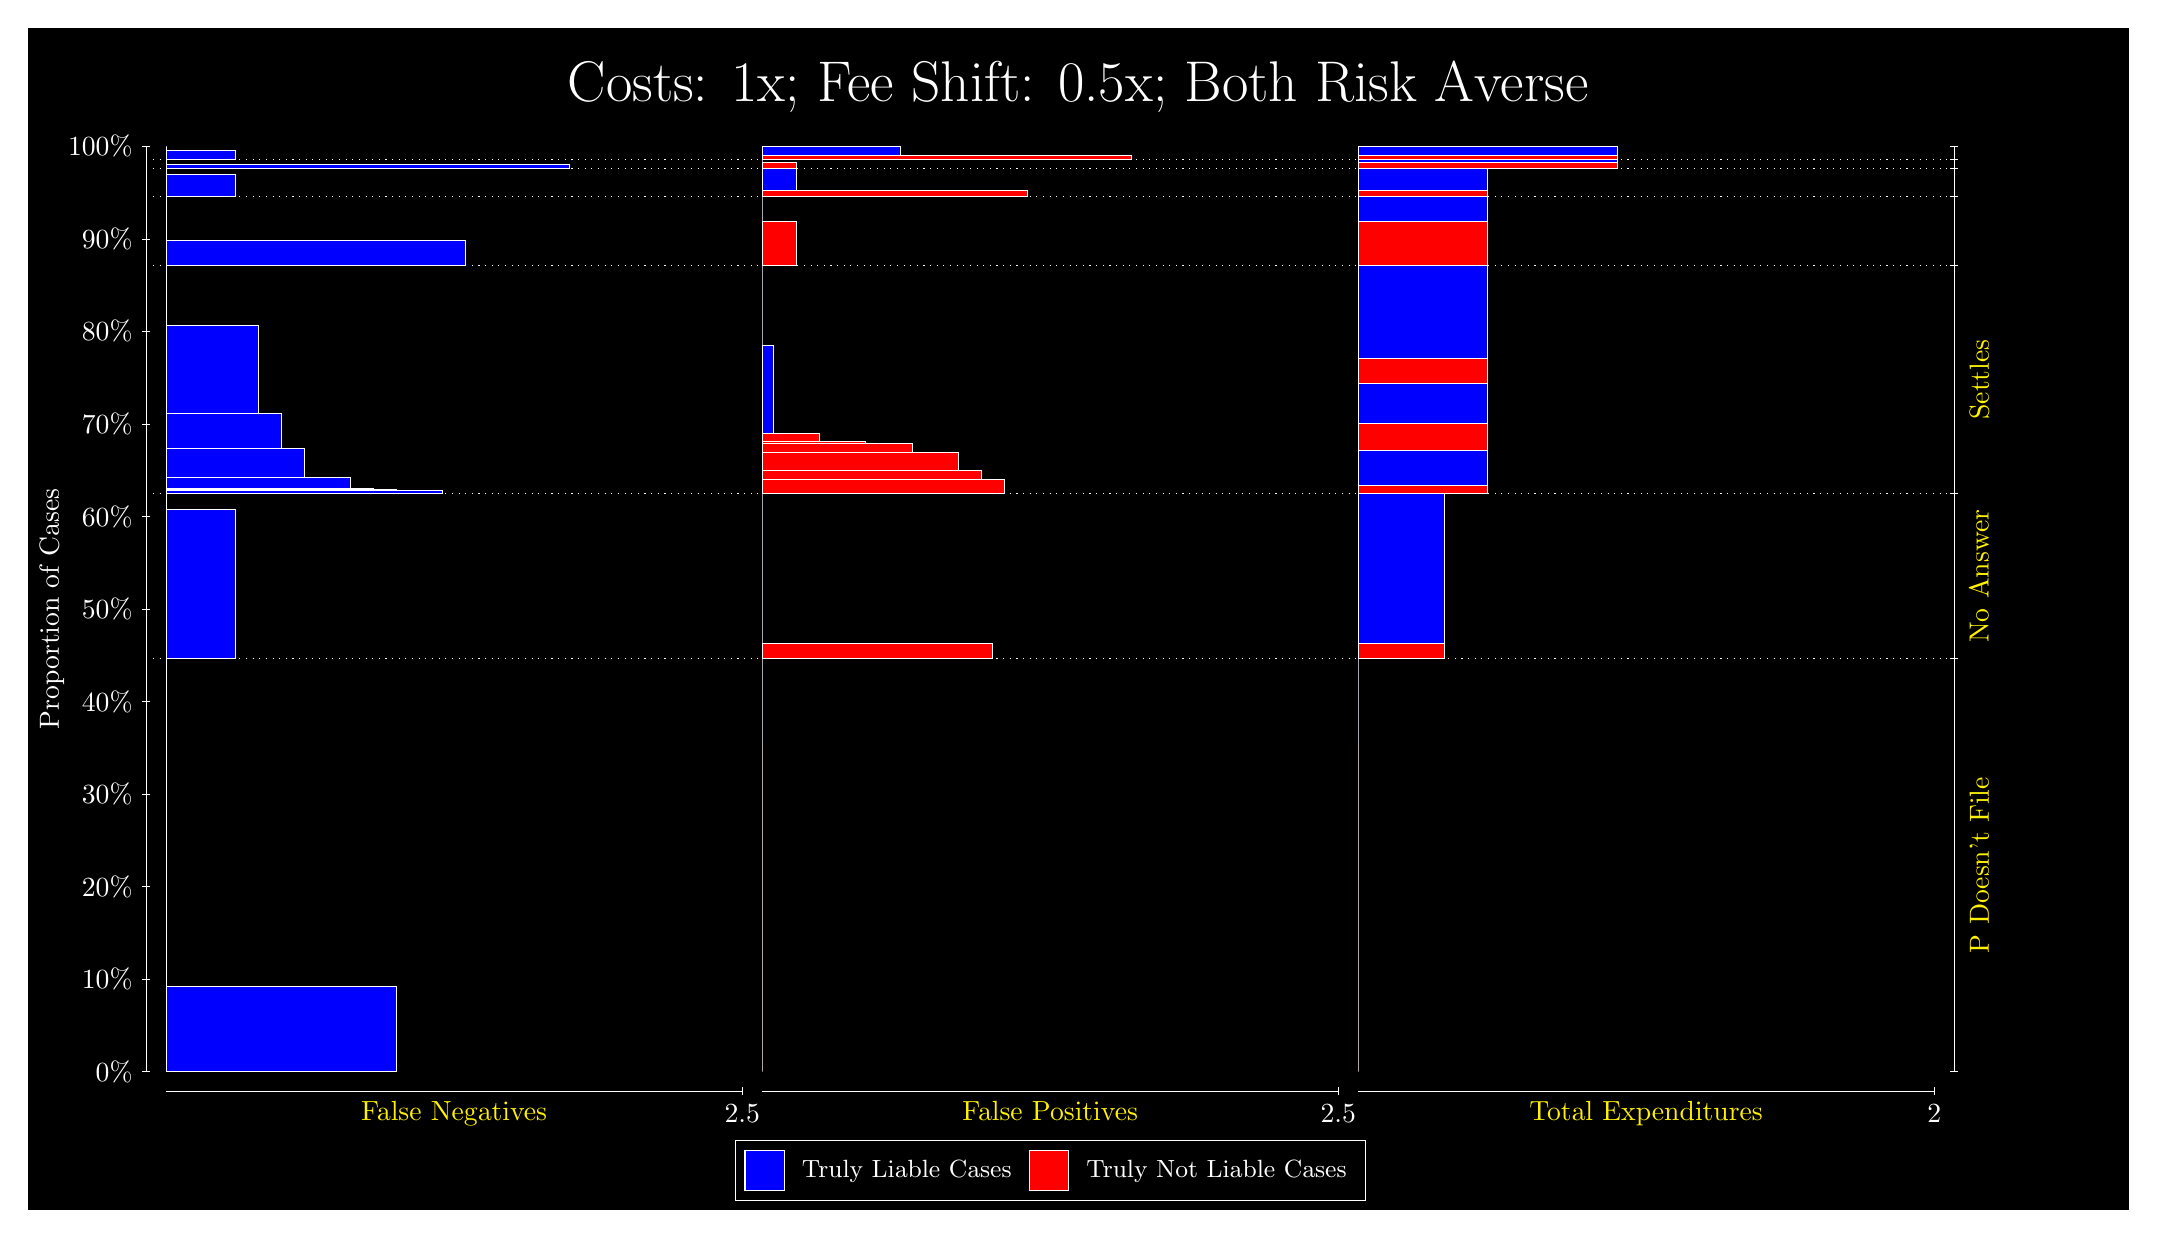
\begin{tikzpicture}
\draw[fill=black] (0,0) rectangle (26.667,15);
\draw[text=white] (0,13.5) rectangle (26.667,15) node[midway] {\huge Costs: 1x; Fee Shift: 0.5x; Both Risk Averse};
\draw[white, very thin] (1.5,1.75) -- (1.5,13.5);
\node[rotate=90, text=white, anchor=center] at (0.3, 7.625) {Proportion of Cases};
\draw[white, very thin] (1.45,1.75) -- (1.55,1.75);
\node[text=white, anchor=east] at (1.45, 1.75) {0\%};
\draw[white, very thin] (1.45,2.925) -- (1.55,2.925);
\node[text=white, anchor=east] at (1.45, 2.925) {10\%};
\draw[white, very thin] (1.45,4.1) -- (1.55,4.1);
\node[text=white, anchor=east] at (1.45, 4.1) {20\%};
\draw[white, very thin] (1.45,5.275) -- (1.55,5.275);
\node[text=white, anchor=east] at (1.45, 5.275) {30\%};
\draw[white, very thin] (1.45,6.45) -- (1.55,6.45);
\node[text=white, anchor=east] at (1.45, 6.45) {40\%};
\draw[white, very thin] (1.45,7.625) -- (1.55,7.625);
\node[text=white, anchor=east] at (1.45, 7.625) {50\%};
\draw[white, very thin] (1.45,8.8) -- (1.55,8.8);
\node[text=white, anchor=east] at (1.45, 8.8) {60\%};
\draw[white, very thin] (1.45,9.975) -- (1.55,9.975);
\node[text=white, anchor=east] at (1.45, 9.975) {70\%};
\draw[white, very thin] (1.45,11.15) -- (1.55,11.15);
\node[text=white, anchor=east] at (1.45, 11.15) {80\%};
\draw[white, very thin] (1.45,12.325) -- (1.55,12.325);
\node[text=white, anchor=east] at (1.45, 12.325) {90\%};
\draw[white, very thin] (1.45,13.5) -- (1.55,13.5);
\node[text=white, anchor=east] at (1.45, 13.5) {100\%};

\draw[white, very thin] (24.457,1.75) -- (24.457,13.5);
\draw[white, very thin] (24.407,1.75) -- (24.507,1.75);
\node[anchor=west] at (24.407, 1.75) {};
\draw[white, very thin] (24.407,6.993) -- (24.507,6.993);
\node[anchor=west] at (24.407, 6.993) {};
\draw[white, very thin] (24.407,9.0896) -- (24.507,9.0896);
\node[anchor=west] at (24.407, 9.0896) {};
\draw[white, very thin] (24.407,11.99) -- (24.507,11.99);
\node[anchor=west] at (24.407, 11.99) {};
\draw[white, very thin] (24.407,12.861) -- (24.507,12.861);
\node[anchor=west] at (24.407, 12.861) {};
\draw[white, very thin] (24.407,13.224) -- (24.507,13.224);
\node[anchor=west] at (24.407, 13.224) {};
\draw[white, very thin] (24.407,13.338) -- (24.507,13.338);
\node[anchor=west] at (24.407, 13.338) {};
\draw[white, very thin] (24.407,13.5) -- (24.507,13.5);
\node[anchor=west] at (24.407, 13.5) {};

\draw[white, very thin, fill=blue] (1.75,1.75) rectangle (4.6775,2.8364);
\draw[white, very thin, fill=red] (1.75,2.8364) rectangle (1.75,6.993);
\draw[white, very thin, fill=blue] (1.75,6.993) rectangle (2.6283,8.8891);
\draw[white, very thin, fill=red] (1.75,8.8891) rectangle (1.75,9.0896);
\draw[white, very thin, fill=blue] (1.75,9.0896) rectangle (5.2631,9.1264);
\draw[white, very thin, fill=blue] (1.75,9.1264) rectangle (4.6775,9.1462);
\draw[white, very thin, fill=blue] (1.75,9.1462) rectangle (4.3848,9.156);
\draw[white, very thin, fill=blue] (1.75,9.156) rectangle (4.092,9.2949);
\draw[white, very thin, fill=blue] (1.75,9.2949) rectangle (3.5065,9.6715);
\draw[white, very thin, fill=blue] (1.75,9.6715) rectangle (3.2138,10.109);
\draw[white, very thin, fill=blue] (1.75,10.109) rectangle (2.921,11.228);
\draw[white, very thin, fill=red] (1.75,11.228) rectangle (1.75,11.99);
\draw[white, very thin, fill=blue] (1.75,11.99) rectangle (5.5558,12.302);
\draw[white, very thin, fill=red] (1.75,12.302) rectangle (1.75,12.861);
\draw[white, very thin, fill=blue] (1.75,12.861) rectangle (2.6283,13.141);
\draw[white, very thin, fill=red] (1.75,13.141) rectangle (1.75,13.224);
\draw[white, very thin, fill=blue] (1.75,13.224) rectangle (6.8732,13.269);
\draw[white, very thin, fill=red] (1.75,13.269) rectangle (1.75,13.338);
\draw[white, very thin, fill=blue] (1.75,13.338) rectangle (2.6283,13.454);
\draw[white, very thin, fill=red] (1.75,13.454) rectangle (1.75,13.5);
\draw[white, very thin, fill=red] (9.3189,1.75) rectangle (9.3189,5.9066);
\draw[white, very thin, fill=blue] (9.3189,5.9066) rectangle (9.3189,6.993);
\draw[white, very thin, fill=red] (9.3189,6.993) rectangle (12.246,7.1935);
\draw[white, very thin, fill=blue] (9.3189,7.1935) rectangle (9.3189,9.0896);
\draw[white, very thin, fill=red] (9.3189,9.0896) rectangle (12.393,9.2737);
\draw[white, very thin, fill=red] (9.3189,9.2737) rectangle (12.1,9.3849);
\draw[white, very thin, fill=red] (9.3189,9.3849) rectangle (11.807,9.6127);
\draw[white, very thin, fill=red] (9.3189,9.6127) rectangle (11.222,9.7235);
\draw[white, very thin, fill=red] (9.3189,9.7235) rectangle (10.929,9.7334);
\draw[white, very thin, fill=red] (9.3189,9.7334) rectangle (10.636,9.7531);
\draw[white, very thin, fill=red] (9.3189,9.7531) rectangle (10.051,9.8517);
\draw[white, very thin, fill=blue] (9.3189,9.8517) rectangle (9.4652,10.971);
\draw[white, very thin, fill=blue] (9.3189,10.971) rectangle (9.3189,11.99);
\draw[white, very thin, fill=red] (9.3189,11.99) rectangle (9.758,12.549);
\draw[white, very thin, fill=blue] (9.3189,12.549) rectangle (9.3189,12.861);
\draw[white, very thin, fill=red] (9.3189,12.861) rectangle (12.686,12.944);
\draw[white, very thin, fill=blue] (9.3189,12.944) rectangle (9.758,13.224);
\draw[white, very thin, fill=red] (9.3189,13.224) rectangle (9.758,13.293);
\draw[white, very thin, fill=blue] (9.3189,13.293) rectangle (9.3189,13.338);
\draw[white, very thin, fill=red] (9.3189,13.338) rectangle (14.003,13.384);
\draw[white, very thin, fill=blue] (9.3189,13.384) rectangle (11.075,13.5);
\draw[white, very thin, fill=red] (16.888,1.75) rectangle (16.888,5.9066);
\draw[white, very thin, fill=blue] (16.888,5.9066) rectangle (16.888,6.993);
\draw[white, very thin, fill=red] (16.888,6.993) rectangle (17.986,7.1935);
\draw[white, very thin, fill=blue] (16.888,7.1935) rectangle (17.986,9.0896);
\draw[white, very thin, fill=red] (16.888,9.0896) rectangle (18.534,9.2008);
\draw[white, very thin, fill=blue] (16.888,9.2008) rectangle (18.534,9.6381);
\draw[white, very thin, fill=red] (16.888,9.6381) rectangle (18.534,9.9767);
\draw[white, very thin, fill=blue] (16.888,9.9767) rectangle (18.534,10.492);
\draw[white, very thin, fill=red] (16.888,10.492) rectangle (18.534,10.805);
\draw[white, very thin, fill=blue] (16.888,10.805) rectangle (18.534,11.99);
\draw[white, very thin, fill=red] (16.888,11.99) rectangle (18.534,12.549);
\draw[white, very thin, fill=blue] (16.888,12.549) rectangle (18.534,12.861);
\draw[white, very thin, fill=red] (16.888,12.861) rectangle (18.534,12.944);
\draw[white, very thin, fill=blue] (16.888,12.944) rectangle (18.534,13.224);
\draw[white, very thin, fill=red] (16.888,13.224) rectangle (20.181,13.293);
\draw[white, very thin, fill=blue] (16.888,13.293) rectangle (20.181,13.338);
\draw[white, very thin, fill=red] (16.888,13.338) rectangle (20.181,13.384);
\draw[white, very thin, fill=blue] (16.888,13.384) rectangle (20.181,13.5);
\draw[white, dotted] (1.5,6.993) -- (24.457,6.993);
\draw[white, dotted] (1.5,9.0896) -- (24.457,9.0896);
\draw[white, dotted] (1.5,11.99) -- (24.457,11.99);
\draw[white, dotted] (1.5,12.861) -- (24.457,12.861);
\draw[white, dotted] (1.5,13.224) -- (24.457,13.224);
\draw[white, dotted] (1.5,13.338) -- (24.457,13.338);
\draw[white, very thin] (1.75,1.5) -- (9.0689,1.5);
\node[text=yellow, anchor=north] at (5.4094, 1.5) {False Negatives};
\draw[white, very thin] (9.0689,1.45) -- (9.0689,1.55);
\node[text=white, anchor=north] at (9.0689, 1.45) {2.5};

\draw[white, very thin] (9.3189,1.5) -- (16.638,1.5);
\node[text=yellow, anchor=north] at (12.978, 1.5) {False Positives};
\draw[white, very thin] (16.638,1.45) -- (16.638,1.55);
\node[text=white, anchor=north] at (16.638, 1.45) {2.5};

\draw[white, very thin] (16.888,1.5) -- (24.207,1.5);
\node[text=yellow, anchor=north] at (20.547, 1.5) {Total Expenditures};
\draw[white, very thin] (24.207,1.45) -- (24.207,1.55);
\node[text=white, anchor=north] at (24.207, 1.45) {2};

\node[text=yellow, centered, rotate=90] at (24.777, 4.3715) {P Doesn't File};
\node[text=yellow, centered, rotate=90] at (24.777, 8.0413) {No Answer};
\node[text=yellow, centered, rotate=90] at (24.777, 10.54) {Settles};





\draw (12.978300999999998,1.5) node[draw=none] (baseCoordinate) {};
\begin{scope}[align=center]
        \matrix[scale=0.5, draw=white, below=0.5cm of baseCoordinate, nodes={draw}, column sep=0.1cm]{
            \node[rectangle, draw, minimum width=0.5cm, minimum height=0.5cm, fill=blue] {}; &
            \node[draw=none, font=\small, text=white] (B) {Truly Liable Cases}; &
            \node[rectangle, draw, minimum width=0.5cm, minimum height=0.5cm, fill=red] {}; &
            \node[draw=none, font=\small, text=white] (B) {Truly Not Liable Cases}; \\
            };
\end{scope}

\end{tikzpicture}
\end{document}